% Important: If latex complains about unicode characters,
% please use "\usepackage[utf8x]{inputenc}" in your preamble
% You can change the size of the picture by putting it into the construct:
% 1) \resizebox{10cm}{!}{"below picture"} to scale horizontally to 10 cm
% 2) \resizebox{!}{15cm}{"below picture"} to scale vertically to 15 cm
% 3) \resizebox{10cm}{15cm}{"below picture"} a combination of above two
% It is not recomended to use the scale option of the tikzpicture environment.
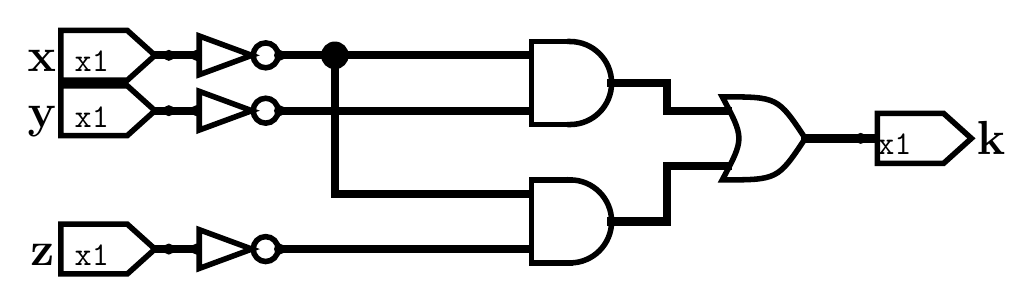
\begin{tikzpicture}[x=1pt,y=-1pt,line cap=rect]
\def\logisimfontA#1{\fontfamily{cmr}{#1}} % Replaced by logisim, original font was "SansSerif"
\def\logisimfontB#1{\fontfamily{cmtt}{#1}} % Replaced by logisim, original font was "Monospaced"
\definecolor{custcol_0_0_0}{RGB}{0, 0, 0}
\definecolor{custcol_ff_ff_ff}{RGB}{255, 255, 255}
\draw [line width=3.0pt, custcol_0_0_0 ]  (96.0,35.0) -- (186.0,35.0) ;
\draw [line width=3.0pt, custcol_0_0_0 ]  (96.0,85.0) -- (186.0,85.0) ;
\draw [line width=3.0pt, custcol_0_0_0 ]  (286.0,45.0) -- (306.0,45.0) ;
\draw [line width=3.0pt, custcol_0_0_0 ]  (116.0,15.0) -- (186.0,15.0) ;
\draw [line width=3.0pt, custcol_0_0_0 ]  (96.0,15.0) -- (116.0,15.0) -- (116.0,65.0) -- (186.0,65.0) ;
\fill [line width=3.0pt, custcol_0_0_0]  (116.0,15.0) ellipse (5.0 and 5.0 );
\draw [line width=3.0pt, custcol_0_0_0 ]  (310.0,45.0) -- (307.0,45.0) ;
\draw [line width=2.0pt, custcol_0_0_0 ]  (336.0,36.0) -- (346.0,45.0) -- (336.0,54.0) -- (312.0,54.0) -- (312.0,36.0) -- cycle;
\logisimfontB{\fontsize{12pt}{12pt}\selectfont\node[inner sep=0, outer sep=0, custcol_0_0_0, anchor=base west] at  (312.0,51.0)  {x1};}
\logisimfontA{\fontsize{16pt}{16pt}\fontseries{bx}\selectfont\node[inner sep=0, outer sep=0, custcol_0_0_0, anchor=base west] at  (348.0,51.0)  {k};}
\fill [line width=2.0pt, custcol_0_0_0]  (306.0,45.0) ellipse (2.0 and 2.0 );
\draw [line width=2.0pt, custcol_0_0_0] (201.0,40.0) arc (90.0:-90.0:15.0 and 15.0 );
\draw [line width=2.0pt, custcol_0_0_0 ]  (201.0,10.0) -- (187.0,10.0) -- (187.0,40.0) -- (201.0,40.0) ;
\draw [line width=3.0pt, custcol_0_0_0 ]  (216.0,25.0) -- (236.0,25.0) -- (236.0,35.0) -- (256.0,35.0) -- (258.0,35.0) ;
\draw [line width=3.0pt, custcol_0_0_0 ]  (216.0,75.0) -- (236.0,75.0) -- (236.0,55.0) -- (256.0,55.0) -- (258.0,55.0) ;
\draw [line width=2.0pt, custcol_0_0_0 ]  (286.0,45.0) .. controls  (276.0,30.0)  ..  (256.0,30.0) .. controls  (264.0,45.0)  ..  (256.0,60.0) .. controls  (276.0,60.0)  ..  (286.0,45.0) -- cycle ;
\draw [line width=2.0pt, custcol_0_0_0] (201.0,90.0) arc (90.0:-90.0:15.0 and 15.0 );
\draw [line width=2.0pt, custcol_0_0_0 ]  (201.0,60.0) -- (187.0,60.0) -- (187.0,90.0) -- (201.0,90.0) ;
\draw [line width=2.0pt, custcol_0_0_0 ]  (86.0,15.0) -- (67.0,8.0) -- (67.0,22.0) -- cycle;
\draw [line width=2.0pt, custcol_0_0_0]  (91.0,15.0) ellipse (4.5 and 4.5 );
\fill [line width=2.0pt, custcol_0_0_0]  (96.0,15.0) ellipse (2.0 and 2.0 );
\fill [line width=2.0pt, custcol_0_0_0]  (66.0,15.0) ellipse (2.0 and 2.0 );
\draw [line width=2.0pt, custcol_0_0_0 ]  (86.0,35.0) -- (67.0,28.0) -- (67.0,42.0) -- cycle;
\draw [line width=2.0pt, custcol_0_0_0]  (91.0,35.0) ellipse (4.5 and 4.5 );
\fill [line width=2.0pt, custcol_0_0_0]  (96.0,35.0) ellipse (2.0 and 2.0 );
\fill [line width=2.0pt, custcol_0_0_0]  (66.0,35.0) ellipse (2.0 and 2.0 );
\draw [line width=3.0pt, custcol_0_0_0 ]  (51.0,35.0) -- (56.0,35.0) -- (66.0,35.0) ;
\draw [line width=2.0pt, custcol_0_0_0 ]  (41.0,44.0) -- (51.0,35.0) -- (41.0,26.0) -- (17.0,26.0) -- (17.0,44.0) -- cycle;
\logisimfontB{\fontsize{12pt}{12pt}\selectfont\node[inner sep=0, outer sep=0, custcol_0_0_0, anchor=base west] at  (22.0,41.0)  {x1};}
\logisimfontA{\fontsize{16pt}{16pt}\fontseries{bx}\selectfont\node[inner sep=0, outer sep=0, custcol_0_0_0, anchor=base west] at  (5.0,41.0)  {y};}
\fill [line width=2.0pt, custcol_0_0_0]  (56.0,35.0) ellipse (2.0 and 2.0 );
\draw [line width=3.0pt, custcol_0_0_0 ]  (51.0,15.0) -- (56.0,15.0) -- (66.0,15.0) ;
\draw [line width=2.0pt, custcol_0_0_0 ]  (41.0,24.0) -- (51.0,15.0) -- (41.0,6.0) -- (17.0,6.0) -- (17.0,24.0) -- cycle;
\logisimfontB{\fontsize{12pt}{12pt}\selectfont\node[inner sep=0, outer sep=0, custcol_0_0_0, anchor=base west] at  (22.0,21.0)  {x1};}
\logisimfontA{\fontsize{16pt}{16pt}\fontseries{bx}\selectfont\node[inner sep=0, outer sep=0, custcol_0_0_0, anchor=base west] at  (5.0,21.0)  {x};}
\fill [line width=2.0pt, custcol_0_0_0]  (56.0,15.0) ellipse (2.0 and 2.0 );
\draw [line width=2.0pt, custcol_0_0_0 ]  (86.0,85.0) -- (67.0,78.0) -- (67.0,92.0) -- cycle;
\draw [line width=2.0pt, custcol_0_0_0]  (91.0,85.0) ellipse (4.5 and 4.5 );
\fill [line width=2.0pt, custcol_0_0_0]  (96.0,85.0) ellipse (2.0 and 2.0 );
\fill [line width=2.0pt, custcol_0_0_0]  (66.0,85.0) ellipse (2.0 and 2.0 );
\draw [line width=3.0pt, custcol_0_0_0 ]  (51.0,85.0) -- (56.0,85.0) -- (66.0,85.0) ;
\draw [line width=2.0pt, custcol_0_0_0 ]  (41.0,94.0) -- (51.0,85.0) -- (41.0,76.0) -- (17.0,76.0) -- (17.0,94.0) -- cycle;
\logisimfontB{\fontsize{12pt}{12pt}\selectfont\node[inner sep=0, outer sep=0, custcol_0_0_0, anchor=base west] at  (22.0,91.0)  {x1};}
\logisimfontA{\fontsize{16pt}{16pt}\fontseries{bx}\selectfont\node[inner sep=0, outer sep=0, custcol_0_0_0, anchor=base west] at  (6.0,91.0)  {z};}
\fill [line width=2.0pt, custcol_0_0_0]  (56.0,85.0) ellipse (2.0 and 2.0 );
\end{tikzpicture}

